\documentclass[12pt]{article}

\usepackage{graphicx}
\usepackage{biblatex}

\title{A (partially-implemented) hydrodynamics code}
\date{\today}
\author{Daniel Boyea}



\begin{document}

\maketitle

\section{Introduction}
Here, I describe some of the structure of the code here, and since the program is heavy on the equations, I also note the critical equations. 

The code is written in Julia

\section{Structure}
The main body of the code is in the \texttt{src/} directory. This directory includes the files
\begin{itemize}
    \item \texttt{GalaxySim.jl}. This just imports and exports other pieces of the project.
    \item \texttt{evolve.jl} contains the main loop of the simulation, including the leapfrog integration scheme and time-step criteria
    \item \verb|gal_files.jl| writes the simulation outputs to files. (Unfortunantly, other io to files for testing are scattered through the project)
    \item \texttt{density.jl} contains routines for density estimation.
    \item \texttt{gravity.jl} calculates the gravity
    \item \texttt{physics.jl} all the rest of the physics (hydrodynaics, viscosity, etc.)
\end{itemize}

\section{Validation}
\begin{figure}
    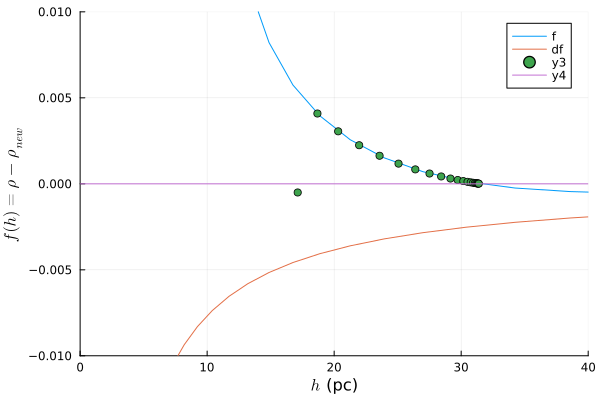
\includegraphics[width=\textwidth]{density.png}
\end{figure}

\end{document}
